\documentclass[12pt]{article}
\usepackage[utf8]{inputenc}
\usepackage[margin=0.75in]{geometry}
\usepackage{array}
\usepackage{tabularx}
\usepackage{pifont}
\usepackage{verbatim}
\usepackage{caption}
\usepackage{cite}
\usepackage{listings}
\usepackage{tikz}

\newcommand{\instbit}[1]{\mbox{\scriptsize #1}}
\newcommand{\instbitrange}[2]{~\instbit{#1} \hfill \instbit{#2}~}
\newcolumntype{I}{>{\centering\arraybackslash}p{0.18in}}
\newcolumntype{W}{>{\centering\arraybackslash}p{0.36in}}
\newcolumntype{F}{>{\centering\arraybackslash}p{0.54in}}
\newcolumntype{Y}{>{\centering\arraybackslash}p{0.72in}}
\newcolumntype{R}{>{\centering\arraybackslash}p{0.9in}}
\newcolumntype{S}{>{\centering\arraybackslash}p{1.08in}}
\newcolumntype{O}{>{\centering\arraybackslash}p{1.26in}}
\newcolumntype{E}{>{\centering\arraybackslash}p{1.44in}}
\newcolumntype{T}{>{\centering\arraybackslash}p{1.8in}}
\newcolumntype{M}{>{\centering\arraybackslash}p{2.2in}}
\newcolumntype{K}{>{\centering\arraybackslash}p{2.88in}}
\newcolumntype{U}{>{\centering\arraybackslash}p{3.6in}}
\newcolumntype{L}{>{\centering\arraybackslash}p{3.6in}}
\newcolumntype{J}{>{\centering\arraybackslash}p{4.5in}}


\newcommand{\wiri}{\textbf{WIRI}}
\newcommand{\wpri}{\textbf{WPRI}}
\newcommand{\wlrl}{\textbf{WLRL}}
\newcommand{\warl}{\textbf{WARL}}

\usetikzlibrary{shapes.geometric}
\tikzstyle{startstop} = [rectangle, rounded corners, minimum width=3cm, minimum height=1cm,text centered, draw=black, fill=red!30]
\tikzstyle{io} = [trapezium, trapezium left angle=70, trapezium right angle=110, minimum width=3cm, minimum height=1cm, text centered, draw=black, fill=blue!30]
\tikzstyle{process} = [rectangle, minimum width=3cm, minimum height=1cm, text centered, draw=black, fill=orange!30]
\tikzstyle{decision} = [diamond, minimum width=3cm, minimum height=1cm, text centered, draw=black, fill=green!30]
\tikzstyle{arrow} = [thick,->,>=stealth]

\title{RISC-V Exceptions and Interrupts}
\author{Sean Keller}
\date{October 2020}

\begin{document}

\maketitle
\newpage

\section{Privilege Modes and Control Status Registers}
RISC-V supports three different privilege modes: M-mode (highest priority), S-mode, and U-mode (lowest priority). Currently, hypervisor-mode (H-mode) is reserved and is not a formal part of the RISC-V ISA. RISC-V also supports an optional debug mode (D-mode) for off-chip debugging that can be considered to be an additional privilege mode with more access than M-mode. Code run in machine-mode (M-mode) is usually inherently trusted, as it has low-level access to the machine implementation. M-mode can be used to manage secure execution environments on RISC-V. User-mode (U-mode) and supervisor-mode (S-mode) are intended for conventional application and operating system usage respectively. Privilege-level actions like exception and interrupt handling rely on a set of control and status registers (CSRs). Each privilege mode supports a set of privilege-specific CSRs for the privilege-specific trap handlers. In this document, CSRs or fields in CSRs prefixed with an \emph{x} refer to the possibility that CSRs can have three privilege-specific implementations: M-mode (x = m), S-mode (x = s), and U-mode (x = u). These privilege-specific CSRs are controlled by their respective privilege-specific trap handlers.

\section{Exceptions and Interrupts}
RISC-V defines exceptions as an unusual condition occurring at run time associated with an instruction in the current hart. Exceptions can be organized into six different categories: fetch, load, store, misaligned jump/branch (i.e misaligned instruction address), illegal instruction, and ECALL/EBREAK. Interrupts refer to an external, asynchronous event that may cause the RISC-V hart to experience an unexpected transfer of control. RISC-V processors must handle each of these exception meaning select exceptions cannot be disabled. Interrupts are organized into three different categories: external, software, and timer. External interrupts are raised by devices connected to the processor, software interrupts are raised by programs, and timer interrupts are raised when the value in the {\tt{xtime}} CSR is greater than or equal the value in the {\tt{xtimecmp}} CSR. For multi-hart systems, interrupts also rely on an inter-processor interface (see Section 6) to handle interrupts between multiple harts. RISC-V processors have the option of handling certain interrupts meaning select interrupts can be enabled or disabled (see Section 6.2). 

\section{Exception Handling}
\subsection{M-Mode Exceptions}
If an exception occurs, control is relinquished by the program that is currently being executed and transferred to the exception handler. The exception handler can be thought of as a software function call the program executes in response to an erroneous hardware event. During this function call the program jumps to an address and writes to a set of CSRs before resuming the program at the location that raised the exception. Before an exception can be raised and handled, the exception handler must be initialized. By default, M-mode, S-mode, and U-mode exceptions are handled by the M-mode exception handler. Software initializes the M-mode exception handler by setting the {\tt{mtvec}} CSR (see Figure \ref{mtvecreg} in the Appendix). The {\tt{mtvec}} CSR contains a base address and a mode field. This mode field supports two options: direct and vectored. For both modes, the program counter is set to the base address in {\tt{mtvec}}. This is where the M-mode exception handler is located.

On entry to the M-mode exception handler, the current execution environment is interrupted and software sets the {\tt{mepc}}, {\tt{mstatus}}, {\tt{mcause}}, and {\tt{mtval}} CSRs before resuming execution at the instruction that raised the exception. The {\tt{mepc}} CSR (see Figure \ref{mepcreg} in the Appendix) is written with the value the program counter was set to for the instruction that took the exception. This value is stored so that the previous execution environment can be returned to and resumed once the exception handler is finished. In M-mode, software changes the MPP, MPIE and MIE fields (see Section 6.2 for more information) in the {\tt{mstatus}} CSR (see Figure \ref{mstatusreg-rv32} in the Appendix). {\tt{mstatus.MPP}} is a 2-bit field that is written with the privilege level encoding that corresponds to the privilege level the program was in when the exception was raised. {\tt{mstatus.MPP}} can hold three values: 11 (M-mode), 01 (S-mode), and 00 (U-mode). {\tt{mstatus.MPIE}} is a 1-bit field that is written with the value the 1-bit, M-mode global interrupt-enable field {\tt{mstatus.MIE}} held when the exception was raised. Once {\tt{mstatus.MPIE}} is written with the value in {\tt{mstatus.MIE}}, the {\tt{mstatus.MIE}} field is set to zero so that the exception handler does not attempt to process an interrupt while the current trap is being handled. The {\tt{mcause}} CSR (see Figure \ref{mcausereg} in the Appendix) is written with the exception cause code that corresponds to the exception that was raised. If an instruction raises multiple synchronous exceptions, the exceptions are taken by the exception handler and reported in {\tt{mcause}} according to a pre-defined priority structure. The {\tt{mtval}} CSR (see Figure \ref{mtvalreg} in the Appendix) is written with exception-specific information. For misaligned addresses, access faults, and page faults, {\tt{mtval}} will contain the faulting virtual address (see Section 4 for more information). Conversely, illegal instructions set {\tt{mtval}} to the faulting instruction whereas EBREAKs and ECALLs set {\tt{mtval}} to zero. If software intends to exit the M-mode exception handler and return to the location that raised the exception after these CSRs are set, it must first determine whether any register states were corrupted during the service routine and resolve these critical errors. Once this is done, software may execute a MRET instruction which sets the program counter to the value stored in {\tt{mepc}} and resumes the previous execution environment. In addition to setting the program counter, MRET also sets {\tt{mstatus.MIE}} to the value in {\tt{mstatus.MPIE}} before setting {\tt{mstatus.MPIE}} to one to indicate that the exception handler is ready for the next interrupt. 

\subsection{S-Mode Exceptions}
Exceptions raised in S-mode can be handled in M-mode or delegated to S-mode through the {\tt{medeleg}} CSR (see Figure \ref{medelegreg} in the Appendix). Delegating to S-mode means that only S-mode CSRs are visible to software and exceptions are processed by the S-mode exception handler. The {\tt{medeleg}} CSR delegates exceptions by raising the bits in positions that correspond to exception code numbers as shown in Figure \ref{medelegcode}. 

\begin{figure}[h!]
{\footnotesize
\begin{center}
\begin{tabular}{MM}
\instbitrange{MXLEN-1}{16} &
\instbitrange{15}{0} \\
\hline
\multicolumn{1}{|c|}{\warl} &
\multicolumn{1}{c|}{Code 15 - Code 0} \\
\hline
MXLEN-16 & 16 \\
\end{tabular}
\end{center}
}
\vspace{-0.1in}
\caption{Machine Exception Delegation Register {\tt medeleg}.}
\label{medelegcode}
\end{figure}

Software initializes the S-mode exception handler by setting the {\tt{stvec}} CSR (see Figure \ref{stvecreg} in the Appendix). The {\tt{stvec}} CSR contains a base address and a mode field. This mode field supports two options: direct and vectored. For both modes, the program counter is set to the base address in {\tt{stvec}}. This is where the S-mode exception handler is located. 

On entry to the S-mode exception handler, the current execution environment is interrupted and software sets the {\tt{sepc}}, {\tt{mstatus}}, {\tt{scause}}, and {\tt{stval}} CSRs before resuming execution at the instruction that raised the exception. The {\tt{sepc}} CSR (see Figure \ref{sepcreg} in the Appendix) is written with the value the program counter was set to for the instruction that took the exception. This value is stored so that the previous execution environment can be returned to and resumed once the exception handler is finished. In S-mode, software changes the SPP, SPIE and SIE fields (see Section 6.2 for more information) in the {\tt{mstatus}}\footnote[1]{S-mode and U-mode can utilize {\tt{mstatus}} instead of {\tt{sstatus}} and {\tt{ustatus}}. These CSRs simply restrict the higher privilege level fields from being visible to hardware.} CSR. {\tt{mstatus.SPP}} is a 1-bit field that is written with the privilege level encoding that corresponds to the privilege level the program was in when the exception was raised. {\tt{mstatus.SPP}} can hold two values: 1 (S-mode) and 0 (U-mode). {\tt{mstatus.SPIE}} is a 1-bit field that is written with the value the 1-bit, S-mode global interrupt-enable field {\tt{mstatus.SIE}} held when the exception was raised. Once {\tt{mstatus.SPIE}} is written with the value in {\tt{mstatus.SIE}}, the {\tt{mstatus.SIE}} field is set to zero so that the exception handler does not attempt to process an interrupt while the current trap is being handled. The {\tt{scause}} CSR (see Figure \ref{scausereg} in the Appendix) is written with the exception cause code that corresponds to the exception that was raised. If an instruction raises multiple synchronous exceptions, the exceptions are taken by the exception handler and reported in {\tt{scause}} according to a pre-defined priority structure. The {\tt{stval}} CSR (see Figure \ref{stvalreg} in the Appendix) is written with exception-specific information. For misaligned addresses, access faults, and page faults, {\tt{stval}} will contain the faulting virtual address (see Section 4 for more information). Conversely, illegal instructions set {\tt{stval}} to the faulting instruction whereas EBREAKs and ECALLs set {\tt{stval}} to zero. If software intends to exit the S-mode exception handler and return to the location that raised the exception after these CSRs are set, it must first determine whether any register states were corrupted during the service routine and resolve these critical errors. Once this is done, software may execute a SRET instruction which sets the program counter to the value stored in {\tt{sepc}} and resumes the previous execution environment. In addition to setting the program counter, SRET also sets {\tt{mstatus.SIE}} to the value in {\tt{mstatus.SPIE}} before setting {\tt{mstatus.SPIE}} to one to indicate that the exception handler is ready for the next interrupt. 

\subsection{U-Mode Exceptions}
Exceptions raised in U-mode can be handled in M-mode, delegated to S-mode through the {\tt{medeleg}} CSR, or delegated to U-mode through the {\tt{sedeleg}} CSR (see Figure \ref{sedelegreg} in the Appendix). Delegating to U-mode means that only U-mode CSRs are visible to software and exceptions are processed by the U-mode exception handler as shown in Figure \ref{delegation}. The {\tt{sedeleg}} CSR delegates exceptions that first must be delegated by the {\tt{medeleg}} CSR by raising the bits in positions that correspond to exception code numbers as shown in Figure \ref{sedelegcode}. 

\begin{figure}[h!]
{\footnotesize
\begin{center}
\begin{tabular}{MM}
\instbitrange{SXLEN-1}{16} &
\instbitrange{15}{0} \\
\hline
\multicolumn{1}{|c|}{0} &
\multicolumn{1}{c|}{Code 15 - Code 0} \\
\hline
SXLEN-16 & 16 \\
\end{tabular}
\end{center}
}
\vspace{-0.1in}
\caption{Machine Exception Delegation Register {\tt sedeleg}.}
\label{sedelegcode}
\end{figure}

Software initializes the U-mode exception handler by setting the {\tt{utvec}} CSR (see Figure \ref{utvecreg} in the Appendix). The {\tt{utvec}} CSR contains a base address and a mode field. This mode field supports two options: direct and vectored. For both modes, the program counter is set to the base address in {\tt{utvec}}. This is where the U-mode exception handler is located.

On entry to the U-mode exception handler, the current execution environment is interrupted and software sets the {\tt{uepc}}, {\tt{mstatus}}, {\tt{ucause}}, and {\tt{utval}} CSRs before resuming execution at the instruction that raised the exception. The {\tt{uepc}} CSR (see Figure \ref{uepcreg} in the Appendix) is written with the value the program counter was set to for the instruction that took the exception. This value is stored so that the previous execution environment can be returned to and resumed once the exception handler is finished. In U-mode, software changes the UPIE and UIE fields (see Section 6.2 for more information) in the {\tt{mstatus}} CSR. The {\tt{mstatus}} CSR does not include a UPP field for U-mode since it is implicitly set to zero. {\tt{mstatus.UPIE}} is a 1-bit field that is written with the value the 1-bit, S-mode global interrupt-enable field {\tt{mstatus.UIE}} held when the exception was raised. Once {\tt{mstatus.UPIE}} is written with the value in {\tt{mstatus.UIE}}, the {\tt{mstatus.UIE}} field is set to zero so that the exception handler does not attempt to process an interrupt while the current trap is being handled. The {\tt{ucause}} CSR (see Figure \ref{ucausereg} in the Appendix) is written with the exception cause code that corresponds to the exception that was raised. If an instruction raises multiple synchronous exceptions, the exceptions are taken by the exception handler and reported in {\tt{ucause}} according to a pre-defined priority structure. The {\tt{utval}} CSR (see Figure \ref{utvalreg} in the Appendix) is written with exception-specific information. For misaligned addresses, access faults, and page faults, {\tt{utval}} will contain the faulting virtual address (see Section 4 for more information). Conversely, illegal instructions set {\tt{utval}} to the faulting instruction whereas EBREAKs and ECALLs set {\tt{utval}} to zero. If software intends to exit the U-mode exception handler and return to the location that raised the exception after these CSRs are set, it must first determine whether any register states were corrupted during the service routine and resolve these critical errors. Once this is done, software may execute a URET instruction which sets the program counter to the value stored in {\tt{uepc}} and resumes the previous execution environment. In addition to setting the program counter, URET also sets {\tt{mstatus.UIE}} to the value in {\tt{mstatus.UPIE}} before setting {\tt{mstatus.UPIE}} to one to indicate that the exception handler is ready for the next interrupt. 

\begin{figure}[h!]
\centering
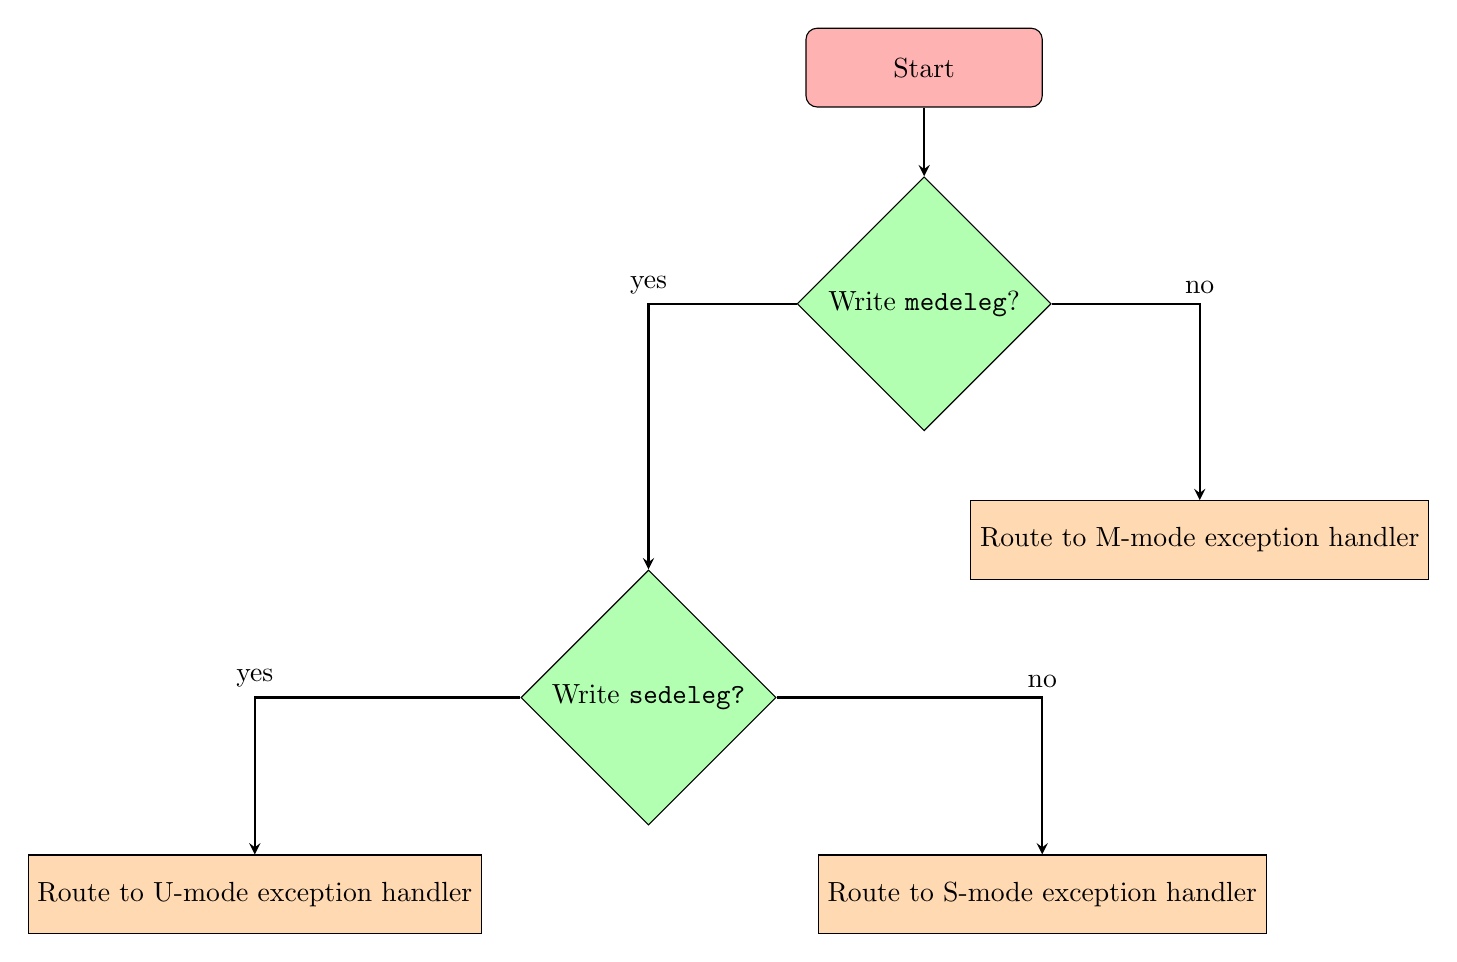
\begin{tikzpicture}[node distance=2cm]
\node (start1) [startstop] {Start};
\node (dec1) [decision, below of=start1, yshift =-1cm] {Write {\tt{medeleg}}?};
\node (pro1) [process, below of=dec1, xshift=3.5cm, yshift=-1cm] {Route to M-mode exception handler};
\node (dec2) [decision, below of=dec1, xshift=-3.5cm, yshift=-3cm] {Write {\tt{sedeleg?}}};
\node (pro2) [process, below of=dec2, xshift=5cm, yshift=-0.5cm] {Route to S-mode exception handler};
\node (pro3) [process, below of=dec2, xshift=-5cm, yshift=-0.5cm] {Route to U-mode exception handler};

\draw [arrow] (start1) -- (dec1);
\draw [arrow] (dec1) -| node[anchor=south] {no} (pro1);
\draw [arrow] (dec1) -| node[anchor=south] {yes} (dec2);
\draw [arrow] (dec2) -| node[anchor=south] {no} (pro2);
\draw [arrow] (dec2) -| node[anchor=south] {yes} (pro3);
\end{tikzpicture}
\caption{Flow Chart of Delegation Process}
\label{delegation}
\end{figure}

\subsection{Exception Priority}
If an instruction raises multiple synchronous exceptions, the decreasing priority order of Table \ref{exceptionpriorities} indicates which exception is taken. Synchronous exceptions are of lower priority than all interrupts and the priority of any custom synchronous exceptions is implementation-defined. 

\begin{table}[h!]
\centering
\begin{tabular}{| l | l | l |}
\hline
Priority & Exception Code & Description \\
\hline
\emph{Highest} & 12 & Instruction Page Fault \\
\hline
& 1 & Instruction Access Fault \\
\hline
& 2 & Illegal Instruction \\ 
\hline
& 0 & Instruction Address Misaligned \\ 
\hline
& 8, 9, 11 & Environment Call (U, S, M) \\
\hline
& 3 & Environment Break \\ 
\hline
& 6 & Store/AMO Address Misaligned \\ 
\hline
& 4 & Load Address Misaligned \\ 
\hline
& 15 & Store/AMO Page Fault \\
\hline
& 13 & Load Page Fault \\
\hline
& 7 & Store/AMO Access Fault \\
\hline
\emph{Lowest} & 5 & Load Access Fault \\ 
\hline
\end{tabular}
\caption{Exception Fault Ordering}
\label{exceptionpriorities}
\end{table}

\section{Exception Definitions}
\subsection{Misaligned Addresses}
Misaligned instruction addresses is a misleading term that refers to misaligned branch and jump targets. The misaligned instruction address should be called misaligned branch/jump target. Misaligned instruction addresses are raised when the target of a jump or branch instruction is not aligned to a 4-byte boundary or an 8-byte boundary. 4-byte alignments are associated with RV32 systems and 8-byte alignments are associated with RV64 systems. 2-byte alignments are also possible for 16-bit instruction implementations but this is a customer instruction encoding that is not a formal part of the RISC-V ISA. Misaligned loads/store addresses are raised when the data the load/store instruction accesses from memory is not aligned to the correct byte offset. In general, a data of size \emph{s} bytes at byte address \emph{A} is aligned if \emph{A} mod \emph{s} = 0.

\subsection{Access Faults}
Instruction, load, and store/AMO access faults are raised from failed physical memory protection checks. Physical memory protection (PMP) checks verify that the instruction is accessed from a valid address in memory by the hardware. Access fault exceptions rely on bits L, X, R, and W in an 8-bit PMP configuration register. Bits X, R, and W encode execute, read, and write privileges respectively. The L-bit indicates that the PMP entry is locked, i.e., writes to the configuration register (see Figure \ref{pmpcfg} in the Appendix) and associated address registers are ignored. In addition to locking the PMP entry, the L bit indicates whether the R/W/X permissions are enforced on M-mode accesses. When the L bit is set, these permissions are enforced for all privilege modes. When the L bit is clear, any M-mode access matching the PMP entry will succeed and the R/W/X permissions only apply to S and U modes. Access fault exceptions can only be raised if the L-bit is set or the access is in S-mode or U-mode. Attempting to fetch an instruction whose physical address lies in a PMP region that does not have execute permissions (X = 0) raises a fetch access exception. Attempting to execute a load or load-reserved instruction whose physical address lies within a PMP region without read permissions (R = 0) raises a load access exception. Attempting to execute a store, store-conditional (regardless of success), or AMO instruction whose physical address lies within a PMP region without write permissions (W = 0) raises a store access exception.

\subsection{Illegal Instructions}
Illegal instructions are raised by illegal instruction encodings or problems reading from and writing to certain CSRs. The following is a non-exhaustive list of illegal instructions that could be raised:
\begin{itemize}
    \item Instructions with bits [15:0] set to zero, this is a reserved bit pattern
    \item Instructions with bits [ILEN-1:0]\footnote[2]{ILEN is the maximum length of the maximum instruction length supported by an implementation. For RISC-V, ILEN is typically 32 or 64 bits.} set to one, this a reserved bit pattern 
    \item Bit patterns that the processor does not recognize (ex. multiply or divide)
    \item Instructions that set rd = x0 with the exception of CSRRW, CSRRWI, JALR, and JAL
    \item Attempts to write to a read-only CSR 
    \item Attempts to access CSRs from non-exsistent CSR addresses
    \item Attempts to access a CSR without appropriate privilege level permissions 
    \item Machine-mode access of debug-mode CSRs
    \item Attempts to read or write the {\tt{satp}} CSR or execute the SFENCE.VMA instruction while executing in S-mode when the TVM bit in the {\tt{xstatus.TVM}} = 1
    \item Attempts to execute the WFI privilege instruction in any less-privileged mode, and it does not complete within an implementation-specific, bounded time limit\footnote[3]{The time limit may \underline{always} be zero, in which case WFI always causes an illegal instruction exception in less-privileged modes when {\tt{mstatus.TW}} equals one} when {\tt{mstatus.TW}} = 1
    \item Attempts to execute SRET while executing in S-mode when {\tt{xstatus.TSR}} = 1
    \item Any instruction that attempts to read or write when {\tt{mstatus.XS[1:0]}} = 0
    \item Attempts to read to the counter registers that correspond to the IR, TM, and CY bits in the {\tt{mcounteren}} CSR when executing in a less-privileged mode 
\end{itemize}

\subsection{Environment Call and Environment Break}
The environment call instruction (ECALL) is used to make a request to the supporting execution environment. When executed in U-mode, S-mode, or M-mode, it generates an environment-call-from-U-mode exception, environment-call-from-S-mode exception, or environment-call-from-M-mode exception, respectively, and performs no other operation. Similarly, the environment break instruction (EBREAK) raises an exception as part of the instruction execution.

\subsection{Page Faults}
For RV32 systems, the supervisor has a 32-bit, page-based virtual memory system called Sv32. RISC-V identifies three different types of page faults: instruction, load, and store/AMO. Instruction page faults are raised by attempting to fetch an instruction from a page that does not have execute permissions. Load page faults are raised by load or load-reserved instructions whose address lies within a page without read permissions. Store/AMO page faults are raised by store, store-conditional, or AMO instruction whose effective address lies within a page without write permissions. In other words, all instructions can raise instruction page faults, load instructions can only raise load page faults, and store instruction can only raise store page faults. This means that load and store page faults also raise instruction page faults. 

The following lists a number of error that can raise a page fault exception that corresponds to the original access type (instruction, load, and store) during the Sv32 virtual to physical address translation process:
\begin{itemize}
    \item The physical address of the page is insufficiently aligned
    \item PTE.V = 0, or PTE.R = 0 and PTE.W = 1
    \item R, W, and X are zero when the page walk is on level two
    \item Accessing a page in U-mode when the PTE.U != 1
    \item Attempting to execute S-mode code on page where the PTE bit U = 1
    \item Attempting to execute loads from pages where R = 0 and X = 0 for {\tt{mstatus.MXR}} = 1
    \item S-mode accesses of pages that are accessible in U-mode (U = 1) when {\tt{mstatus.SUM}} = 0
    \item PTE.A = 0, or if the memory access is a store and PTE.D = 0
\end{itemize}

\section{Exception Table}
The exceptions in Table \ref{exceptiontable} fall under the following categories fetch, load, store, misaligned branch/jump, rd != x0 illegal instruction, and ECALL/EBREAK. Fetch exceptions encompass instruction access faults and instruction page faults. Load exceptions encompass misaligned load addresses, load access faults, and load page faults. Store exceptions encompass misaligned store addresses, store access faults, and store page faults. Unless otherwise specified, the fetch, store, and load categories encompass all the respective exceptions included in each category. Misaligned branch/jump exceptions are raised by jump and branch instructions according to the definition for misaligned instruction addresses. EBREAK/ECALL exceptions are raised according to the definitions of environment call and environment break.

\begin{table}
\centering
\begin{tabular}{| c || c | c | c | c | c | c |} 
\hline
Instruction & Fetch & Load & Store & Misaligned Branch/Jump & rd != x0 & ECALL/EBREAK \\
\hline
LUI & \ding{53} & & & & \ding{53} & \\
\hline
AUIPC & \ding{53} & & & & \ding{53} & \\
\hline
JAL & \ding{53} & & & \ding{53} & & \\
\hline
JALR & \ding{53} & & & \ding{53} & & \\
\hline
BEQ & \ding{53} & & & \ding{53} & & \\
\hline
BNE & \ding{53} & & & \ding{53} & & \\
\hline
BLT & \ding{53} & & & \ding{53} & & \\
\hline
BGE & \ding{53} & & & \ding{53} & & \\
\hline
BLTU & \ding{53} & & & \ding{53} & & \\
\hline
BGEU & \ding{53} & & & \ding{53} & & \\
\hline
LB & \ding{53} & \ding{53} & & & \ding{53} & \\
\hline
LH & \ding{53} & \ding{53} & & & \ding{53} & \\
\hline
LW & \ding{53} & \ding{53} & & & \ding{53} & \\
\hline
LBU & \ding{53} & \ding{53} & & & \ding{53} & \\
\hline
LHU & \ding{53} & \ding{53} & & & \ding{53} & \\
\hline
SB & \ding{53} & & \ding{53} & & & \\
\hline
SH & \ding{53} & & \ding{53} & & & \\
\hline
SW & \ding{53} & & \ding{53} & & & \\
\hline
ADDI & \ding{53} & & & & \ding{53} & \\
\hline
SLTI & \ding{53} & & & & \ding{53} & \\
\hline
SLTIU & \ding{53} & & & & \ding{53} & \\
\hline
XORI & \ding{53} & & & & \ding{53} & \\
\hline
ORI & \ding{53} & & & & \ding{53} & \\
\hline
ANDI & \ding{53} & & & & \ding{53} & \\
\hline
SLLI & \ding{53} & & & & \ding{53} & \\
\hline
SRLI & \ding{53} & & & & \ding{53} & \\
\hline
SRAI & \ding{53} & & & & \ding{53} & \\
\hline
ADD & \ding{53} & & & & \ding{53} & \\
\hline
SUB & \ding{53} & & & & \ding{53} & \\
\hline
SLL & \ding{53} & & & & \ding{53} & \\
\hline
SLT & \ding{53} & & & & \ding{53} & \\
\hline
SLTU & \ding{53} & & & & \ding{53} & \\
\hline
XOR & \ding{53} & & & & \ding{53} & \\
\hline
SRL & \ding{53} & & & & \ding{53} & \\
\hline
SRA & \ding{53} & & & & \ding{53} & \\
\hline
OR & \ding{53} & & & & \ding{53} & \\
\hline
AND & \ding{53} & & & & \ding{53} & \\
\hline
ECALL & \ding{53} & & & & & \ding{53} \\
\hline
EBREAK & \ding{53} & & & & & \ding{53} \\
\hline
\end{tabular}
\caption{Possible Exceptions for the RV32I Instruction Set}
\label{exceptiontable}
\end{table}

\section{Interrupt Handling}
\subsection{PLIC, CLINT, and CLIC}
Interrupt handling is similar to exception handling but there are some notable differences. Unlike exceptions, interrupts require additional hardware. This additional hardware includes a RISC-V Platform Level Interrupt Controller (PLIC)\cite{PLIC} and the option of a SiFive Core-local Interrupter (CLINT)\cite{CLINT} or a RISC-V Core-local Interrupt Controller (CLIC)\cite{CLIC}. The PLIC sources external interrupts from devices and routes them to the hart(s) as shown in Figure \ref{PLIC_CLINT}. Similarly, the CLINT sources local software and timer interrupts and routes them to the hart(s). Unlike the CLINT, the CLIC routes external, software, and timer interrupt signals to the hart(s) as shown in Figure \ref{PLIC_CLIC}. RISC-V has defined detailed CLIC and PLIC specifications that explain the interrupt control flow and define the different registers that are used to handle interrupts. For systems with multiple harts, the Wait for Interrupt (WFI) instruction can be implemented to control interrupt servicing between multiple harts by stalling a hart. If an enabled interrupt is present or later becomes present while the hart is stalled, the interrupt exception will be taken on the following instruction.

\begin{figure}[h!]
    \centering
    \includegraphics[scale=0.8]{PLIC and CLINT Block Diagram.JPG}
    \caption{Block diagram of an example PLIC and CLINT configuration}
    \label{PLIC_CLINT}
\end{figure}
\begin{figure}[h!]
    \centering
    \includegraphics[scale=0.8]{PLIC and CLIC Block Diagram.JPG}
    \caption{Block diagram of an example PLIC and CLIC configuration}
    \label{PLIC_CLIC}
\end{figure}

\subsection{Interrupt Control Flow}
Unlike exceptions, interrupts do not depend on synchronous hardware problems in the processor. Instead, interrupts are asynchronous events external to the processor that are driven devices, timers, or software. Before information about interrupts can be routed from the interrupt controllers to the processor, they must be globally and locally enabled. Global interrupt enables are controlled by the {\tt{mstatus.xie}} fields and the current privilege mode. M-mode interrupts are globally enabled if the current privilege mode is less than M or the current privilege mode is M and {\tt{mstatus.MIE}} = 1. S-mode interrupts are globally enabled if the current privilege mode is less the S or the current privilege mode is S and {\tt{mstatus.SIE}} = 1. U-mode interrupts are globally enabled if the current privilege mode is U and {\tt{mstatus.UIE}} = 1. Local interrupts are controlled by the {\tt{mie}} CSR (see Figure \ref{miereg} in the Appendix). External interrupts in M-mode, S-mode, and U-mode are enabled by raising the 1-bit {\tt{mie.MEIE}}, {\tt{mie.SEIE}}, and {\tt{mie.UEIE}} fields respectively. Timer interrupts in M-mode, S-mode, and U-mode are enabled by raising the 1-bit {\tt{mie.MTIE}}, {\tt{mie.STIE}}, and {\tt{mie.UTIE}} fields respectively. Software interrupts in M-mode, S-mode, and U-mode are enabled by raising the 1-bit {\tt{mie.MSIE}}, {\tt{mie.SSIE}}, and {\tt{mie.USIE}} fields respectively. 

Once the selected interrupts are globally and locally enabled, the interrupt controllers are responsible for identifying pending interrupts and raising the appropriate fields in the {\tt{mip}} CSR (see Figure \ref{mipreg} in the Appendix). M-mode external, software, and timer interrupts are raised by setting the 1-bit {\tt{mip.MEIP}}, {\tt{mip.MSIP}}, and {\tt{mip.MTIP}} fields respectively. S-mode external, software, and timer interrupts are raised by setting the 1-bit {\tt{mip.SEIP}}, {\tt{mip.SSIP}}, and {\tt{mip.STIP}} fields respectively. U-mode external, software, and timer interrupts are raised by setting the 1-bit {\tt{mip.UEIP}}, {\tt{mip.USIP}}, and {\tt{mip.UTIP}} fields respectively. 

\subsection{M-Mode Interrupts}
If M-mode, S-mode, or U-mode bits in {\tt{mip}} are raised, control is relinquished by the program that is currently being executed and transferred to an interrupt handler. By default, M-mode, S-mode, and U-mode interrupts are handled by the M-mode interrupt handler. Software initializes the M-mode interrupt handler by setting the {\tt{mtvec}} CSR. The {\tt{mtvec}} CSR contains a base address and a mode field. This mode field supports two options: direct and vectored. In direct mode, the program counter is set to the base address in {\tt{mtvec}}. For vectored mode, the program counter is set to the base address plus four times the interrupt cause code as shown in Table \ref{interruptvectors}\footnote[4]{When vectored interrupts are enabled, interrupt cause 0, which corresponds to user-mode software interrupts, are vectored to the same location as synchronous exceptions. This ambiguity does not arise in practice, since user-mode software interrupts are either disabled or delegated to a less-privileged mode.}. This can be thought of as a jump table that contains different jump targets for interrupt-specific handling routines. Once the M-mode interrupt handler is initialized, interrupts are processed in the same manner as exceptions as specified in Section 3.1. The only difference is that interrupts do not set {\tt{mtval}} and it is therefore left cleared.

\begin{table}[h!]
\centering
\begin{tabular}{| l | l |}
\hline
Interrupt & BASE + $4*cause$ \\
\hline
User Software Interrupt & BASE \\
\hline
Supervisor Software Interrupt & BASE + 0x4 \\
\hline
\emph{Reserved} & BASE + 0x8 \\ 
\hline
Machine Software Interrupt & BASE + 0xC \\ 
\hline
User Timer Interrupt & BASE + 0x10 \\
\hline
Supervisor Timer Interrupt & BASE + 0x14 \\ 
\hline
\emph{Reserved} & BASE + 0x18 \\ 
\hline
Machine Timer Interrupt & BASE + 0x1C \\ 
\hline
User External Interrupt & BASE + 0x20 \\ 
\hline
Supervisor External Interrupt & BASE + 0x24 \\ 
\hline
\emph{Reserved} & BASE + 0x28 \\ 
\hline
Machine External Interrupt & BASE + 0x2C \\ 
\hline
\end{tabular}
\caption{Interrupt Vector Table}
\label{interruptvectors}
\end{table}

\subsection{S-Mode Interrupts}
If M-mode, S-mode, or U-mode bits in {\tt{mip}} are raised, control is relinquished by the program that is currently being executed and transferred to an interrupt handler. Interrupts raised in S-mode can be handled in M-mode or delegated to S-mode through the {\tt{mideleg}} CSR. Delegating to S-mode means that only S-mode CSRs are visible in hardware and interrupts are processed by the S-mode interrupt handler. The S-mode interrupt handler can process S-mode and U-mode interrupts. Software initializes the S-mode interrupt handler by setting the {\tt{stvec}} CSR. The {\tt{stvec}} CSR contains a base address and a mode field. This mode field supports two options: direct and vectored. In direct mode, the program counter is set to the base address in {\tt{stvec}}. For vectored mode, the program counter is set to the base address plus four times the interrupt cause code. This can be thought of as a jump table that contains different jump targets for interrupt-specific handling routines. Once the S-mode interrupt handler is initialized, interrupts processed by the S-mode interrupt handler are processed in the same manner as exceptions as specified in Section 3.2. The only difference is that interrupts do not set {\tt{stval}} and it is therefore left cleared. 

\subsection{U-Mode Interrupts}
If M-mode, S-mode, or U-mode bits in {\tt{mip}} are raised, control is relinquished by the program that is currently being executed and transferred to an interrupt handler. Interrupts raised in U-mode can be handled in M-mode, delegated to S-mode through the {\tt{mideleg}} CSR, or delegated to U-mode through the \emph{sideleg} CSR. Delegating to U-mode means that only U-mode CSRs are visible in hardware and interrupts are processed by the U-mode interrupt handler. The U-mode interrupt handler can only process U-mode interrupts. Software initializes the U-mode interrupt handler by setting the {\tt{utvec}} CSR. The {\tt{utvec}} CSR contains a base address and a mode field. This mode field supports two options: direct and vectored. In direct mode, the program counter is set to the base address in {\tt{utvec}}. For vectored mode, the program counter is set to the base address plus four times the interrupt cause code. This can be thought of as a jump table that contains different jump targets for interrupt-specific handling routines. Once the M-mode interrupt handler is initialized, interrupts processed by the U-mode interrupt handler are processed in the same manner as exceptions as specified in Section 3.3. The only difference is that interrupts do not set {\tt{utval}} and it is therefore left cleared.

\subsection{Interrupt Priority}
Like exceptions, simultaneous interrupts are processed by the interrupt handler according to a fixed priority structure as show in Table \ref{interruptpriorities}. The exception codes for interrupts are differentiated from the exception codes for exceptions with a 1-bit interrupt field in the MSB of {\tt{xcause}}. Raising this field indicates that the exception code in {\tt{xcause}} is for an interrupt. 

\begin{table}[h!]
\centering
\begin{tabular}{| l | l | l |}
\hline
Priority & Exception Code & Description \\
\hline
\emph{Highest} & 11 & Machine External Interrupt \\
\hline
& 3 & Machine Software Interrupt \\
\hline
& 7 & Machine Timer Interrupt \\ 
\hline
& 9 & Supervisor External Interrupt \\ 
\hline
& 1 & Supervisor Software Interrupt \\
\hline
& 5 & Supervisor Timer Interrupt \\ 
\hline
& 8 & User External Interrupt \\ 
\hline
& 0 & User Software Interrupt \\ 
\hline
\emph{Lowest} & 4 & User Timer Interrupt \\ 
\hline
\end{tabular}
\caption{Interrupt Priorities}
\label{interruptpriorities}
\end{table}

\clearpage

\section{CSR Appendix}

\begin{figure*}[h!]
{\footnotesize
\begin{center}
\begin{tabular}{J@{}S}
\instbitrange{MXLEN-1}{2} &
\instbitrange{1}{0} \\
\hline
\multicolumn{1}{|c|}{BASE[MXLEN-1:2]} & 
\multicolumn{1}{c|}{MODE} \\
\hline
MXLEN-2 & 2 \\
\end{tabular}
\end{center}
}
\vspace{-0.1in}
\caption{Machine trap-vector base-address register ({\tt mtvec}).}
\label{mtvecreg}
\end{figure*}

\begin{figure}[h!]
{\footnotesize
\begin{center}
\begin{tabular}{@{}J}
\instbitrange{MXLEN-1}{0} \\
\hline
\multicolumn{1}{|c|}{\tt mepc} \\
\hline
MXLEN \\
\end{tabular}
\end{center}
}
\vspace{-0.1in}
\caption{Machine exception program counter register.}
\label{mepcreg}
\end{figure}

\begin{figure*}[h!]
{\footnotesize
\begin{center}
\setlength{\tabcolsep}{4pt}
\begin{tabular}{cKccccccc}
\\
\instbit{31} &
\instbitrange{30}{23} &
\instbit{22} &
\instbit{21} &
\instbit{20} &
\instbit{19} &
\instbit{18} &
\instbit{17} &
 \\
\hline
\multicolumn{1}{|c|}{SD} &
\multicolumn{1}{c|}{\emph{Reserved}} &
\multicolumn{1}{c|}{TSR} &
\multicolumn{1}{c|}{TW} &
\multicolumn{1}{c|}{TVM} &
\multicolumn{1}{c|}{MXR} &
\multicolumn{1}{c|}{SUM} &
\multicolumn{1}{c|}{MPRV} &
 \\
\hline
1 & 8 & 1 & 1 & 1 & 1 & 1 & 1 & \\
\end{tabular}
\begin{tabular}{cWWcWccccccccc}
\\
&
\instbitrange{16}{15} &
\instbitrange{14}{13} &
\instbitrange{12}{11} &
\instbitrange{10}{9} &
\instbit{8} &
\instbit{7} &
\instbit{6} &
\instbit{5} &
\instbit{4} &
\instbit{3} &
\instbit{2} &
\instbit{1} &
\instbit{0} \\
\hline
 &
\multicolumn{1}{|c|}{XS[1:0]} &
\multicolumn{1}{c|}{FS[1:0]} &
\multicolumn{1}{c|}{MPP[1:0]} &
\multicolumn{1}{c|}{\emph{Reserved}} &
\multicolumn{1}{c|}{SPP} &
\multicolumn{1}{c|}{MPIE} &
\multicolumn{1}{c|}{\emph{Reserved}} &
\multicolumn{1}{c|}{SPIE} &
\multicolumn{1}{c|}{UPIE} &
\multicolumn{1}{c|}{MIE} &
\multicolumn{1}{c|}{\emph{Reserved}} &
\multicolumn{1}{c|}{SIE} &
\multicolumn{1}{c|}{UIE} \\
\hline
 & 2 & 2 & 2 & 2 & 1 & 1 & 1 & 1 & 1 & 1 & 1 & 1 & 1 \\
\end{tabular}
\end{center}
}
\vspace{-0.1in}
\caption{Machine-mode status register ({\tt mstatus}) for RV32.}
\label{mstatusreg-rv32}
\end{figure*}

\begin{figure}[h!]
{\footnotesize
\begin{center}
\begin{tabular}{@{}J}
\instbitrange{MXLEN-1}{0} \\
\hline
\multicolumn{1}{|c|}{\tt mtval} \\
\hline
MXLEN \\
\end{tabular}
\end{center}
}
\vspace{-0.1in}
\caption{Machine Trap Value register.}
\label{mtvalreg}
\end{figure}

\begin{figure*}[h!]
{\footnotesize
\begin{center}
\begin{tabular}{c@{}U}
\instbit{MXLEN-1} &
\instbitrange{MXLEN-2}{0} \\
\hline
\multicolumn{1}{|c|}{Interrupt} &
\multicolumn{1}{c|}{Exception Code} \\
\hline
1 & MXLEN-1 \\
\end{tabular}
\end{center}
}
\vspace{-0.1in}
\caption{Machine Cause register {\tt mcause}.}
\label{mcausereg}
\end{figure*}

\begin{figure}[h!]
{\footnotesize
\begin{center}
\begin{tabular}{@{}U}
\instbitrange{MXLEN-1}{0} \\
\hline
\multicolumn{1}{|c|}{Synchronous Exceptions} \\
\hline
MXLEN \\
\end{tabular}
\end{center}
}
\vspace{-0.1in}
\caption{Machine Exception Delegation Register {\tt medeleg}.}
\label{medelegreg}
\end{figure}

\begin{figure*}[h!]
{\footnotesize
\begin{center}
\begin{tabular}{J@{}R}
\instbitrange{SXLEN-1}{2} &
\instbitrange{1}{0} \\
\hline
\multicolumn{1}{|c|}{BASE[SXLEN-1:2]} & 
\multicolumn{1}{c|}{MODE} \\
\hline
SXLEN-2 & 2 \\
\end{tabular}
\end{center}
}
\vspace{-0.1in}
\caption{Supervisor trap vector base address register ({\tt stvec}).}
\label{stvecreg}
\end{figure*}

\begin{figure}[h!]
{\footnotesize
\begin{center}
\begin{tabular}{@{}J}
\instbitrange{SXLEN-1}{0} \\
\hline
\multicolumn{1}{|c|}{\tt sepc} \\
\hline
SXLEN \\
\end{tabular}
\end{center}
}
\vspace{-0.1in}
\caption{Supervisor exception program counter register.}
\label{sepcreg}
\end{figure}

\begin{figure}[h!]
{\footnotesize
\begin{center}
\begin{tabular}{@{}J}
\instbitrange{SXLEN-1}{0} \\
\hline
\multicolumn{1}{|c|}{\tt stval} \\
\hline
SXLEN \\
\end{tabular}
\end{center}
}
\vspace{-0.1in}
\caption{Supervisor Trap Value register.}
\label{stvalreg}
\end{figure}

\begin{figure*}[h!]
{\footnotesize
\begin{center}
\begin{tabular}{c@{}U}
\instbit{SXLEN-1} &
\instbitrange{SXLEN-2}{0} \\
\hline
\multicolumn{1}{|c|}{Interrupt} &
\multicolumn{1}{c|}{Exception Code} \\
\hline
1 & SXLEN-1 \\
\end{tabular}
\end{center}
}
\vspace{-0.1in}
\caption{Supervisor Cause register {\tt scause}.}
\label{scausereg}
\end{figure*}

\begin{figure}[h!]
{\footnotesize
\begin{center}
\begin{tabular}{@{}U}
\instbitrange{SXLEN-1}{0} \\
\hline
\multicolumn{1}{|c|}{Synchronous Exceptions} \\
\hline
SXLEN \\
\end{tabular}
\end{center}
}
\vspace{-0.1in}
\caption{Supervisor Exception Delegation Register {\tt sedeleg}.}
\label{sedelegreg}
\end{figure}

\begin{figure*}[h!]
{\footnotesize
\begin{center}
\begin{tabular}{J@{}R}
\instbitrange{UXLEN-1}{2} &
\instbitrange{1}{0} \\
\hline
\multicolumn{1}{|c|}{BASE[UXLEN-1:2]} & 
\multicolumn{1}{c|}{MODE} \\
\hline
UXLEN-2 & 2 \\
\end{tabular}
\end{center}
}
\vspace{-0.1in}
\caption{User trap vector base address register ({\tt utvec}).}
\label{utvecreg}
\end{figure*}

\begin{figure}[h!]
{\footnotesize
\begin{center}
\begin{tabular}{@{}J}
\instbitrange{UXLEN-1}{0} \\
\hline
\multicolumn{1}{|c|}{\tt uepc} \\
\hline
UXLEN \\
\end{tabular}
\end{center}
}
\vspace{-0.1in}
\caption{User exception program counter register.}
\label{uepcreg}
\end{figure}

\begin{figure}[h!]
{\footnotesize
\begin{center}
\begin{tabular}{@{}J}
\instbitrange{UXLEN-1}{0} \\
\hline
\multicolumn{1}{|c|}{\tt utval} \\
\hline
UXLEN \\
\end{tabular}
\end{center}
}
\vspace{-0.1in}
\caption{User Trap Value register.}
\label{utvalreg}
\end{figure}

\begin{figure*}[h!]
{\footnotesize
\begin{center}
\begin{tabular}{c@{}U}
\instbit{UXLEN-1} &
\instbitrange{UXLEN-2}{0} \\
\hline
\multicolumn{1}{|c|}{Interrupt} &
\multicolumn{1}{c|}{Exception Code} \\
\hline
1 & UXLEN-1 \\
\end{tabular}
\end{center}
}
\vspace{-0.1in}
\caption{User Cause register {\tt ucause}.}
\label{ucausereg}
\end{figure*}

\begin{figure}[h!]
{\footnotesize
\begin{center}
\begin{tabular}{cWWccc}
\instbit{7} &
\instbitrange{6}{5} &
\instbitrange{4}{3} &
\instbit{2} &
\instbit{1} &
\instbit{0} \\
\hline
\multicolumn{1}{|c|}{L} &
\multicolumn{1}{c|}{0} &
\multicolumn{1}{c|}{A} &
\multicolumn{1}{c|}{X} &
\multicolumn{1}{c|}{W} &
\multicolumn{1}{c|}{R}
\\
\hline
1 & 2 & 2 & 1 & 1 & 1 \\
\end{tabular}
\end{center}
}
\vspace{-0.1in}
\caption{PMP configuration register format.}
\label{pmpcfg}
\end{figure}

\begin{figure*}[h!]
{\footnotesize
\begin{center}
\setlength{\tabcolsep}{4pt}
\begin{tabular}{Rcccccccccccc}
\instbitrange{MXLEN-1}{12} &
\instbit{11} &
\instbit{10} &
\instbit{9} &
\instbit{8} &
\instbit{7} &
\instbit{6} &
\instbit{5} &
\instbit{4} &
\instbit{3} &
\instbit{2} &
\instbit{1} &
\instbit{0} \\
\hline
\multicolumn{1}{|c|}{0} &
\multicolumn{1}{c|}{MEIE} &
\multicolumn{1}{c|}{0} &
\multicolumn{1}{c|}{SEIE} &
\multicolumn{1}{c|}{0} &
\multicolumn{1}{c|}{MTIE} &
\multicolumn{1}{c|}{0} &
\multicolumn{1}{c|}{STIE} &
\multicolumn{1}{c|}{0} &
\multicolumn{1}{c|}{MSIE} &
\multicolumn{1}{c|}{0} &
\multicolumn{1}{c|}{SSIE} &
\multicolumn{1}{c|}{0} \\
\hline
MXLEN-12 & 1 & 1 & 1 & 1 & 1 & 1 & 1 & 1 & 1 & 1 & 1 & 1 \\
\end{tabular}
\end{center}
}
\vspace{-0.1in}
\caption{Machine Interrupt Enable Register {\tt mie}.}
\label{miereg}
\end{figure*}

\begin{figure*}[h!]
{\footnotesize
\begin{center}
\setlength{\tabcolsep}{4pt}
\begin{tabular}{Rcccccccccccc}
\instbitrange{MXLEN-1}{12} &
\instbit{11} &
\instbit{10} &
\instbit{9} &
\instbit{8} &
\instbit{7} &
\instbit{6} &
\instbit{5} &
\instbit{4} &
\instbit{3} &
\instbit{2} &
\instbit{1} &
\instbit{0} \\
\hline
\multicolumn{1}{|c|}{0} &
\multicolumn{1}{c|}{MEIP} &
\multicolumn{1}{c|}{0} &
\multicolumn{1}{c|}{SEIP} &
\multicolumn{1}{c|}{0} &
\multicolumn{1}{c|}{MTIP} &
\multicolumn{1}{c|}{0} &
\multicolumn{1}{c|}{STIP} &
\multicolumn{1}{c|}{0} &
\multicolumn{1}{c|}{MSIP} &
\multicolumn{1}{c|}{0} &
\multicolumn{1}{c|}{SSIP} &
\multicolumn{1}{c|}{0} \\
\hline
MXLEN-12 & 1 & 1 & 1 & 1 & 1 & 1 & 1 & 1 & 1 & 1 & 1 & 1 \\
\end{tabular}
\end{center}
}
\vspace{-0.1in}
\caption{Machine Interrupt Pending Register {\tt mip}.}
\label{mipreg}
\end{figure*}

\begin{figure}[h!]
{\footnotesize
\begin{center}
\begin{tabular}{@{}U}
\instbitrange{MXLEN-1}{0} \\
\hline
\multicolumn{1}{|c|}{Interrupts} \\
\hline
MXLEN \\
\end{tabular}
\end{center}
}
\vspace{-0.1in}
\caption{Machine Interrupt Delegation Register {\tt mideleg}.}
\label{midelegreg}
\end{figure}

\begin{figure}[h!]
{\footnotesize
\begin{center}
\begin{tabular}{@{}U}
\instbitrange{SXLEN-1}{0} \\
\hline
\multicolumn{1}{|c|}{Interrupts} \\
\hline
SXLEN \\
\end{tabular}
\end{center}
}
\vspace{-0.1in}
\caption{Supervisor Interrupt Delegation Register {\tt sideleg}.}
\label{sidelegreg}
\end{figure}

\clearpage

\bibliographystyle{IEEEtran}
\bibliography{IEEEabrv,bibliography}
\end{document}
